\documentclass[9pt, aspectratio=169]{beamer}
\usepackage{FiraSans}
\usetheme[subsectionpage=progressbar]{metropolis}
\usepackage[utf8]{inputenc}
\usepackage{amsmath}
\usepackage{amsfonts}
\usepackage{amssymb}
\usepackage{multicol}
\usepackage{tikz}
\usetikzlibrary{math, positioning, matrix}
\usepackage{caption}
\usepackage{xcolor}
\usepackage[T1]{fontenc} 
\usepackage[skins]{tcolorbox}
\author{Nicola Roman\`o - nicola.romano@ed.ac.uk}
\title{CNN for segmentation}
\setlength{\fboxsep}{0pt}
\setbeamertemplate {footline}{\begin{scriptsize}\hfill\insertframenumber ~of \inserttotalframenumber\kern1em\vskip5pt\end{scriptsize}}

% Remove "Figure" in front of captions
% See https://tex.stackexchange.com/questions/82456/how-to-remove-figure-caption-prefix-figure-in-beamer
\captionsetup{labelformat=empty,labelsep=none}

\titlegraphic{\centering 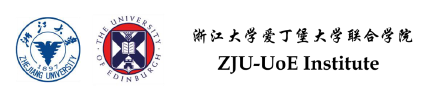
\includegraphics[scale=.5]{instituteLogo.png}}
\date{}

\begin{document}

\newtcolorbox{codebox}{enhanced,
    top=2pt,
    left=2pt,
    right=2pt,
    bottom=2pt,
    boxrule=0pt,
    leftrule=5pt,
    sharp corners,
    colback=gray!20,
    colframe=blue!60!black}

\begin{frame}
    \titlepage
\end{frame}

\begin{frame}
    {In the past few lectures...}
    \begin{itemize}
        \item We discussed ML approaches for image analysis.
        \item We introduced artificial neural networks (ANNs)
        \item We saw how convolutional neural networks (CNNs) can overcome the limitations of ANNs in image analysis.
        \item We discussed strategies for image classification by looking at classic examples (AlexNet, VGG, GoogLeNet, ...).
    \end{itemize}
\end{frame}

\begin{frame}
    {A note on transfer learning}
    \only <1>{
        \begin{itemize}
            \item Training a CNN is expensive in terms of time and computer memory.
            \item Luckily, you can make use of pre-trained models to speed up the training process!
            \item This process is called \textbf{transfer learning}.
            \item For example, if you wanted to classify images, rather than start from scratch you could begin with VGG-16, or with GoogLeNet and modify them for your needs! (i.e. do not reinvent the wheel!)
        \end{itemize}
    }
    \centering
    \begin{tikzpicture}[scale=0.9]
        \only <2->{
            % Generic images
            \node[inner sep=0pt] (generic) at (0,2)
            {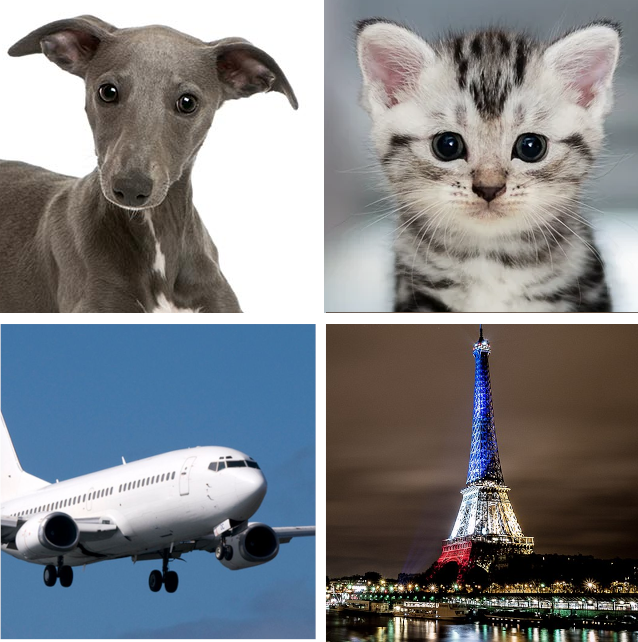
\includegraphics[height=2.5cm]{genericimages.png}};
            \node (label) at (0, 0) {Generic images};

            % Top CNN
            % Conv layers
            \foreach \x [count=\N] in {2.5,3,...,5}
                {
                    \node (layer\N) [draw, rectangle, fill=orange!50!yellow, minimum width=1, minimum height=3cm-0.4*\N cm] at (\x,1.5) {};
                }
            % FC layers
            \foreach \x [count=\N from 7] in {6,6.5,7}
                {
                    \node (layer\N) [draw, rectangle, fill=blue!50!yellow, minimum width=1, minimum height=2.5cm-.1*\N cm] at (\x,1.5) {};
                }
            \node [text width=4em] (layer10) at (9.5, 1.5) {Dog, Cat, Plane, \dots};
            % Arrows
            \foreach \N [count=\Nn from 2] in {1,2,...,9}
                {
                    \draw [->] (layer\N) -- (layer\Nn.west);
                }
            \node [right of=label, node distance=6cm] {\textit{"Template"} CNN - e.g. VGG-16};

            \only<3>{
                % Domain specific images
                \node[inner sep=0pt] (generic) at (0,-2)
                {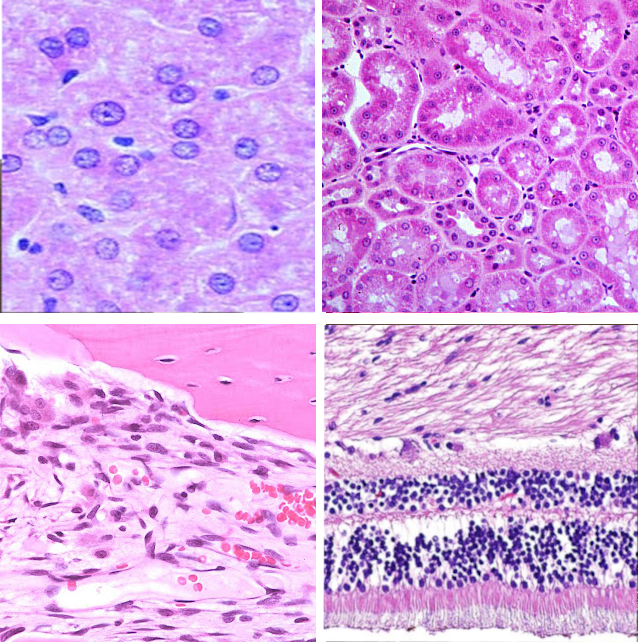
\includegraphics[height=2.5cm]{bioimages.png}};
                \node at (0, -4) {Task-specific images};

                % Bottom CNN
                % Conv layers
                \foreach \x [count=\N] in {2.5,3,...,4.5}
                    {
                        \node (layer_bottom_\N) [draw, rectangle, fill=orange!50!yellow, minimum width=1, minimum height=3cm-0.4*\N cm] at (\x,-2) {};
                    }
                \node (layer_bottom_6) [draw, rectangle, fill=green!40!yellow, minimum width=1, minimum height=0.6cm] at (5,-2) {};

                % FC layers
                \foreach \x [count=\N from 7] in {6,6.5,7}
                    {
                        \node (layer_bottom_\N) [draw, rectangle, fill=green!60!yellow, minimum width=1, minimum height=2.5cm-.1*\N cm] at (\x,-2) {};
                    }

                \node [text width=4em] (layer_bottom_10) at (9.5, -2) {Liver, Kidney, Bone, Retina, \dots};
                \node [color=orange!80!black] at (4, 4) {\textbf{Conv layers}};
                \node [color=blue!50!yellow] at (6.5, 4) {\textbf{FC layers}};
                \draw [color=orange, line width=1pt] (2.2,-3.7) -- (4.8,-3.7) node [below, midway] {Keep};
                \draw [color=green!50!black, line width=1pt] (5,-3.7) -- (8,-3.7) node [below, midway] {Retrain};
                % Arrows
                \foreach \N [count=\Nn from 2] in {1,2,...,9}
                    {
                        \draw [->] (layer_bottom_\N) -- (layer_bottom_\Nn.west);
                    }
            }
        }
    \end{tikzpicture}
\end{frame}

\begin{frame}
    {Learning objectives}
    \begin{columns}
        \begin{column}{0.8\textwidth}
            \begin{itemize}
                \item Define the problems of segmentation, classification, localization and object detection.
                \item Describe CNN-based methods to solve these problems.
                \item Discuss advantages and disadvantages of these methods.
            \end{itemize}
        \end{column}
        \begin{column}{0.2\textwidth}
            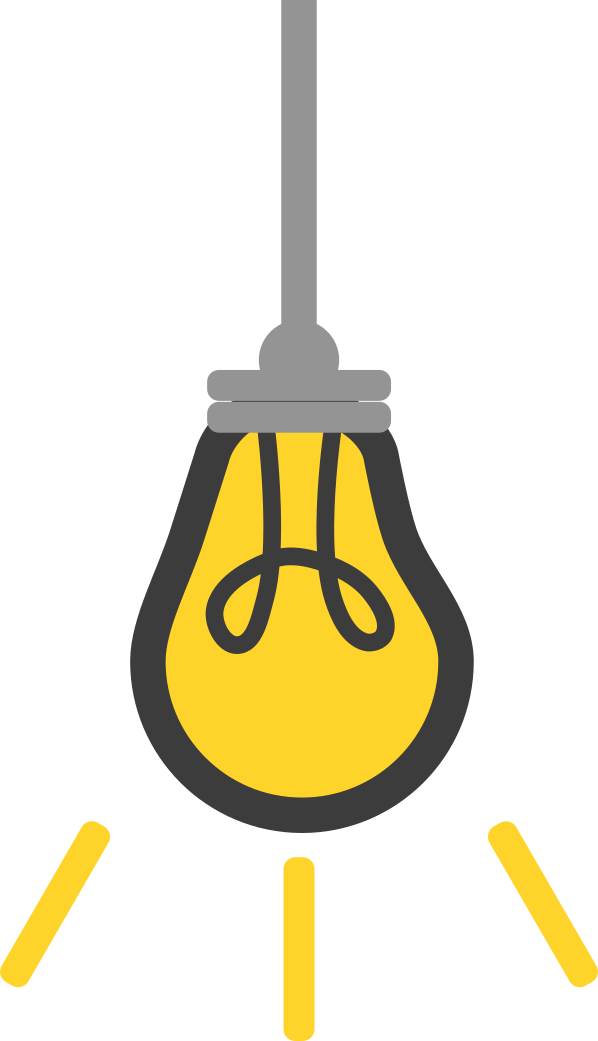
\includegraphics[angle=-30, origin=tr, width=1.5\textwidth]{lightbulb.png}
        \end{column}
    \end{columns}
\end{frame}

\section{Introduction}

\begin{frame}
    {Computer vision problems}
    \begin{columns}[t]
        \begin{column}{.5\textwidth}
            \begin{itemize}
                \item \textbf{Image classification}: determine what class an image belongs to.

                      \centering
                      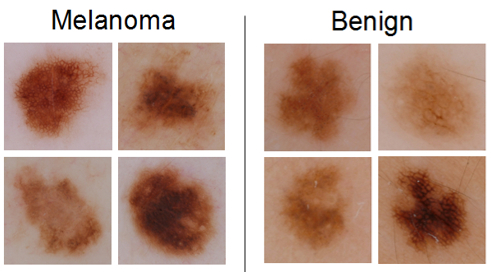
\includegraphics[width=.6\textwidth]{ISIC_melanoma.jpg}
                      \pause
                \item \raggedright \textbf{Segmentation}: dividing an image into groups (segments) of pixels with similar \textit{meaning}.

                      \centering
                      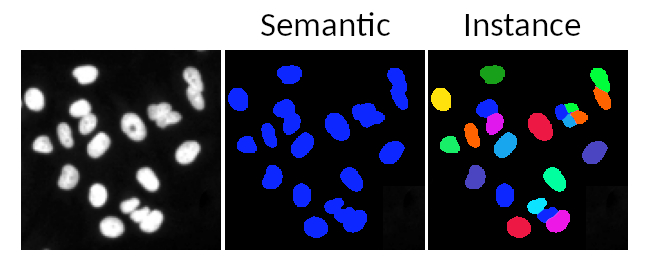
\includegraphics[width=.7\textwidth]{semantic_vs_instance_bio.jpg}
            \end{itemize}
        \end{column}
        \pause
        \begin{column}{.5\textwidth}
            \begin{itemize}
                \item \textbf{Localization}: determine the location (\textbf{bounding box}) of an object in an image.
                      \centering
                      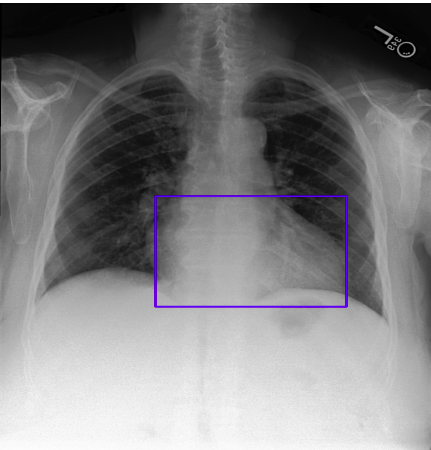
\includegraphics[width=.3\textwidth]{Nkechinyere_2021_localization.png}
                      \raisebox{1cm}{\rotatebox[origin=t]{-90}{\footnotesize Nkechinyere et al. 2021}}
                      \pause
                \item \raggedright \textbf{Detection}: Detecting the location of objects in an image, and classifying them.
                      \centering
                      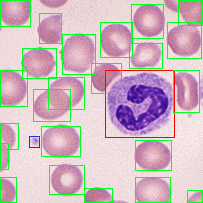
\includegraphics[width=.4\textwidth]{objectdetection.png}
            \end{itemize}
        \end{column}
    \end{columns}
\end{frame}

\section{Using CNN for segmentation}

\begin{frame}
    {So far...}
    So far we've looked into CNNs for image classification

    \centering
    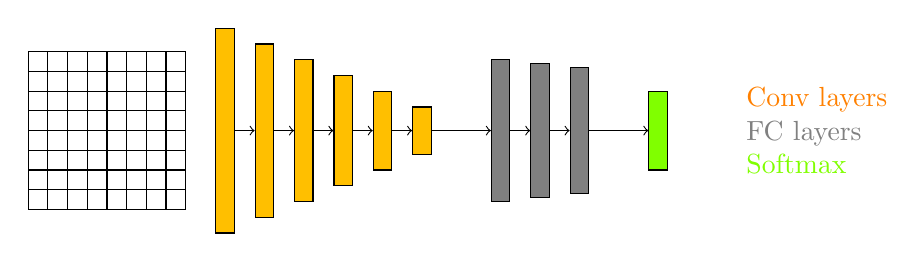
\begin{tikzpicture}
        \draw (0, 0.5) rectangle ++(2, 2) grid [step=0.25] ++(-2, -2);

        % Conv layers
        \foreach \x [count=\N] in {2.5,3,...,5}
            {
                \node (layer\N) [draw, rectangle, fill=orange!50!yellow, minimum width=1, minimum height=3cm-0.4*\N cm] at (\x,1.5) {};
            }
        % FC layers
        \foreach \x [count=\N from 7] in {6,6.5,7}
            {
                \node (layer\N) [draw, rectangle, fill=blue!50!yellow, minimum width=1, minimum height=2.5cm-.1*\N cm] at (\x,1.5) {};
            }

        % Softmax
        \node (layer10) [draw, rectangle, fill=green!50!yellow, minimum width=1, minimum height=1cm] at (8,1.5) {};

        % Arrows
        \foreach \N [count=\Nn from 2] in {1,2,...,9}
            {
                \draw [->] (layer\N) -- (layer\Nn.west);
            }

        \node [text width=5em] at (10, 1.5) {\color{orange}{\mbox{Conv layers}} \color{blue!50!yellow}{\mbox{FC layers}} \color{green!50!yellow}{\mbox{Softmax}}};
    \end{tikzpicture}

    \raggedright
    To segment an image, we need to use a different architecture, with an output that matches the input image.

    \textbf{How to do that?}
\end{frame}

\begin{frame}
    {A na\"ive approach (don't do this!)}
    We could reduce the segmentation problem to a classification problem using a sliding window going over each pixel and then through a CNN.

    \vspace{2em}
    \centering
    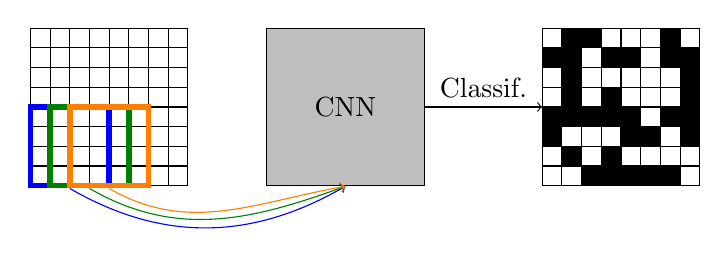
\begin{tikzpicture}
        % Image
        \draw [fill=white] (0, 0) rectangle ++(2,2) grid [step=0.25] (0,0);

        \node (pixel1) [draw, color=blue, line width=2pt, minimum size=1cm] at (0.5, 0.5) {};
        \node (pixel2) [draw, color=green!50!black, line width=2pt, minimum size=1cm] at (0.75, 0.5) {};
        \node (pixel3) [draw, color=orange, line width=2pt, minimum size=1cm] at (1, 0.5) {};

        % CNN       
        \node (CNN) [draw, rectangle, fill=lightgray, minimum size=2cm] at (4, 1) {CNN};

        % Arrows
        \draw [color=blue, ->] (pixel1.south) to [out=-30, in=210] (CNN.south);
        \draw [color=green!50!black, ->] (pixel2.south) to [out=-30, in=200] (CNN.south);
        \draw [color=orange, ->] (pixel3.south) to [out=-30, in=190] (CNN.south);

        % Output image
        \foreach \y in {0.0,0.25,...,1.75}
            {
                \foreach \x in {6.5,6.75,...,8.25}
                    {
                        \pgfmathparse{round(rnd)}
                        \definecolor{MyColor}{rgb}{\pgfmathresult,\pgfmathresult,\pgfmathresult}
                        \path[fill=MyColor] (\x,\y) rectangle ++(0.25,0.25);
                    }
            }

        \draw (6.5, 0) rectangle ++(2,2) grid [step=0.25] (6.5,0);

        \draw [->] (CNN.east) -- (6.5,1) node [above, midway, align=center] {Classif.};
    \end{tikzpicture}

    \pause

    \begin{itemize}
        \item Slow and computationally intensive
        \item Inefficient: we reuse information from the same pixel multiple times
    \end{itemize}
\end{frame}

\begin{frame}
    {A better convolutional-only approach}
    We can use a series of same convolutions to keep image size, then use $1\times 1$ convolutions to reduce the layer depth to the desired number of classes $c$.

    \centering
    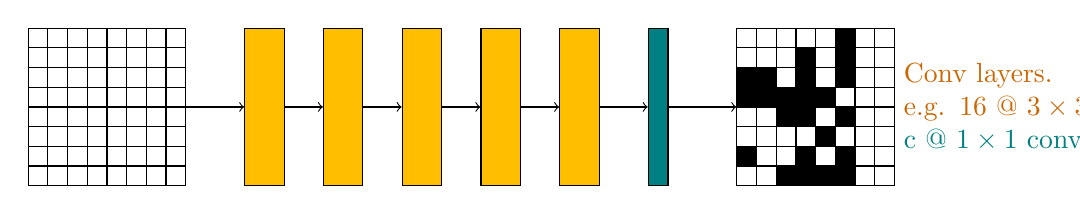
\begin{tikzpicture}
        % Image
        \node (input) [draw, rectangle, minimum size = 2cm] at (1, 1) {};
        \draw (2, 2) grid [step=0.25] (0,0);

        % Conv layers
        \foreach \x [count=\N] in {3,4,...,7}
            {
                \node (layer\N) [draw, rectangle, fill=orange!50!yellow, minimum width=0.5cm, minimum height=2cm] at (\x,1) {};
            }

        \node (layer6) [draw, rectangle, fill=blue!50!green, minimum width=0.25cm, minimum height=2cm] at (8,1) {};

        % Arrows
        \draw [->] (input) -- (layer1.west);
        \foreach \N [count=\Nn from 2] in {1,2,...,5}
            {
                \draw [->] (layer\N) -- (layer\Nn.west);
            }

        % Output
        \foreach \y in {0.0,0.25,...,1.75}
            {
                \foreach \x in {9,9.25,...,10.25}
                    {
                        \pgfmathparse{round(rnd)}
                        \definecolor{MyColor}{rgb}{\pgfmathresult,\pgfmathresult,\pgfmathresult}
                        \path[fill=MyColor] (\x,\y) rectangle ++(0.25,0.25);
                    }
            }

        \node (output) [draw, rectangle, minimum size = 2cm] at (10, 1) {};
        \draw (11, 2) grid [step=0.25] (9,0);
        \draw [->] (layer6.east) -- (output);

        % Labels
        \node [text width=5em] at (12, 1) {\color{orange!80!black}{\mbox{Conv layers.} \mbox{e.g. 16 $@~3\times 3$}} \color{blue!50!green}{\mbox{c $@~1\times 1$ conv}}};
    \end{tikzpicture}

    \pause
    \begin{itemize}
        \item Faster and more efficient
        \item Still a lot of calculations (same convolutions, no pooling), so problematic for big images
    \end{itemize}
\end{frame}

\begin{frame}
    {A much better and usable solution!}
    \centering
    \textbf{\Large Downscale, then upscale!}
    \normalsize
    \vspace {2em}

    \centering
    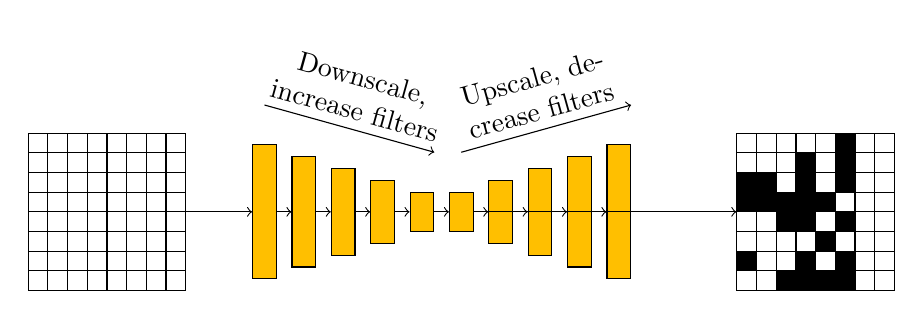
\begin{tikzpicture}
        % Image
        \node (input) [draw, rectangle, minimum size = 2cm] at (1, 1) {};
        \draw (2, 2) grid [step=0.25] (0,0);

        % Conv layers
        \foreach \x [count=\N] in {3,3.5,...,5}
            {
                \node (layer\N) [draw, rectangle, fill=orange!50!yellow, minimum width=0.3cm, minimum height=2cm - \N * 0.3 cm] at (\x,1) {};
            }
        \foreach \x [count=\N from 6] in {5.5,6,...,7.5}
            {
                \pgfmathsetmacro{\Nn}{(11 - \N)*0.3}
                \node (layer\N) [draw, rectangle, fill=orange!50!yellow, minimum width=0.3cm, minimum height=2cm - \Nn cm] at (\x,1) {};
            }

        % Arrows
        \draw [->] (input) -- (layer1.west);
        \foreach \N [count=\Nn from 2] in {1,2,...,9}
            {
                \draw [->] (layer\N) -- (layer\Nn.west);
            }

        % Output
        \foreach \y in {0.0,0.25,...,1.75}
            {
                \foreach \x in {9,9.25,...,10.25}
                    {
                        \pgfmathparse{round(rnd)}
                        \definecolor{MyColor}{rgb}{\pgfmathresult,\pgfmathresult,\pgfmathresult}
                        \path[fill=MyColor] (\x,\y) rectangle ++(0.25,0.25);
                    }
            }

        \node (output) [draw, rectangle, minimum size = 2cm] at (10, 1) {};
        \draw (11, 2) grid [step=0.25] (9,0);
        \draw [->] (layer6.east) -- (output);

        \draw [->] ([yshift=0.5cm]layer1.north) -- ([yshift=0.5cm]layer5.north east) node [above, align=center, midway, sloped, text width=8em] {Downscale, increase filters};
        \draw [->] ([yshift=0.5cm]layer6.north) -- ([yshift=0.5cm]layer10.north east) node [above, align=center, midway, sloped, text width=8em] {Upscale, decrease filters};

    \end{tikzpicture}

    \pause

    Advantages:
    \begin{itemize}
        \item Convolutional only system
        \item Most of the processing is done at a small spatial scale, so it is faster
        \item The downscaling path helps determining the "what" while the upscale path helps determining the "where".
    \end{itemize}
\end{frame}

\begin{frame}
    {Upscaling - non-learnable}
    Simple ideas for upscaling include \textbf{nearest neighbor interpolation}, \textbf{bilinear interpolation}, or "\textbf{bed of nails}" approaches.

    \centering

    \only <1> {
        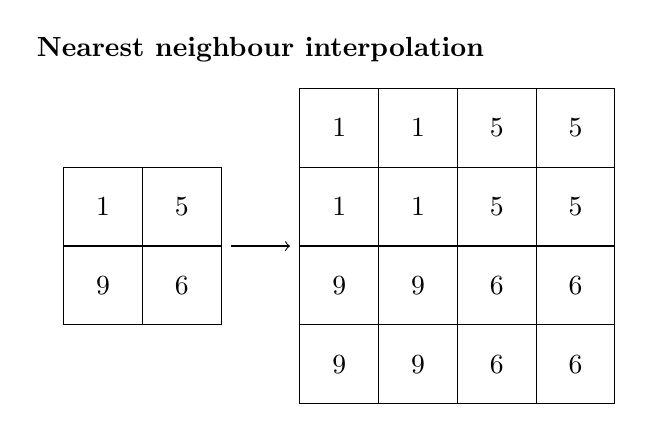
\begin{tikzpicture}
            % Nearest neighbours
            \node [align=center] at (1.5, 2.5) {\textbf{Nearest neighbour interpolation}};
            \draw [fill=white] (-1,-1) rectangle ++(2,2) [step=1] grid ++(-2,-2);

            \matrix (m1) [matrix of nodes, ampersand replacement=\&, nodes={anchor=center, minimum size=1cm}] at (0, 0)
            {
                1 \& 5 \\
                9 \& 6 \\
            };

            \draw [fill=white] (2,-2) rectangle ++(4,4) [step=1] grid ++(-4,-4);

            \matrix (m2) [matrix of nodes, ampersand replacement=\&, nodes={anchor=center, minimum size=1cm}] at (4, 0)
            {
                1 \& 1 \& 5 \& 5 \\
                1 \& 1 \& 5 \& 5 \\
                9 \& 9 \& 6 \& 6 \\
                9 \& 9 \& 6 \& 6 \\
            };

            \draw [->] (m1) -- (m2);
        \end{tikzpicture}
    }

    \only <2> {
        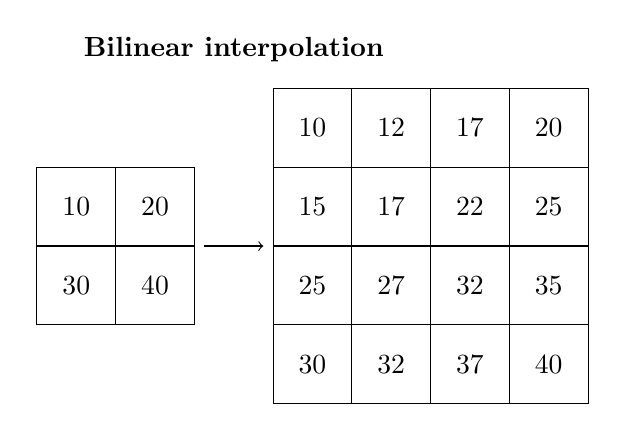
\begin{tikzpicture}
            % Bilinear neighbours
            \node [align=center] at (1.5, 2.5) {\textbf{Bilinear interpolation}};
            \draw [fill=white] (-1,-1) rectangle ++(2,2) [step=1] grid ++(-2,-2);

            \matrix (m1) [matrix of nodes, ampersand replacement=\&, nodes={anchor=center, minimum size=1cm}] at (0, 0)
            {
                10 \& 20 \\
                30 \& 40 \\
            };

            \draw [fill=white] (2,-2) rectangle ++(4,4) [step=1] grid ++(-4,-4);

            \matrix (m2) [matrix of nodes, ampersand replacement=\&, nodes={anchor=center, minimum size=1cm}] at (4, 0)
            {
                10 \& 12 \& 17 \& 20 \\
                15 \& 17 \& 22 \& 25 \\
                25 \& 27 \& 32 \& 35 \\
                30 \& 32 \& 37 \& 40 \\
            };

            \draw [->] (m1) -- (m2);
        \end{tikzpicture}
    }

    \only <3> {
        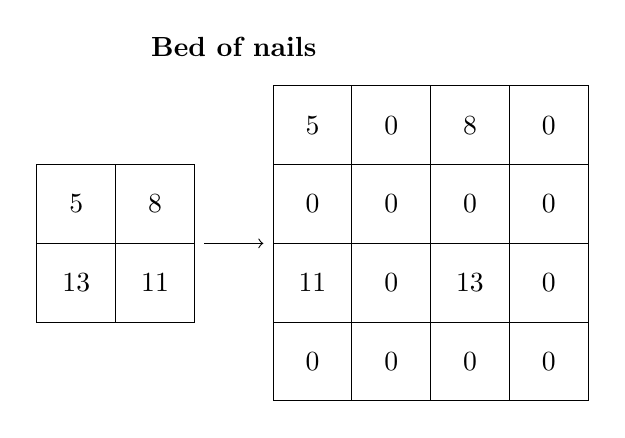
\begin{tikzpicture}
            % "Bed of nails"
            \node [align=center] at (1.5, 2.5) {\textbf{Bed of nails}};
            \draw [fill=white] (-1,-1) rectangle ++(2,2) [step=1] grid ++(-2,-2);

            \matrix (m1) [matrix of nodes, ampersand replacement=\&, nodes={anchor=center, minimum size=1cm}] at (0, 0)
            {
                5 \& 8   \\
                13 \& 11 \\
            };

            \draw [fill=white] (2,-2) rectangle ++(4,4) [step=1] grid ++(-4,-4);

            \matrix (m2) [matrix of nodes, ampersand replacement=\&, nodes={anchor=center, minimum size=1cm}] at (4, 0)
            {
                5 \& 0 \& 8 \& 0   \\
                0 \& 0 \& 0 \& 0   \\
                11 \& 0 \& 13 \& 0 \\
                0 \& 0 \& 0 \& 0   \\
            };

            \draw [->] (m1) -- (m2);
        \end{tikzpicture}
    }
\end{frame}

\begin{frame}
    {Upscaling - learnable}
    A learnable approach to upscaling is \textbf{transpose convolutions}. The value of each pixel is used as a scaler for a learnable filter.

    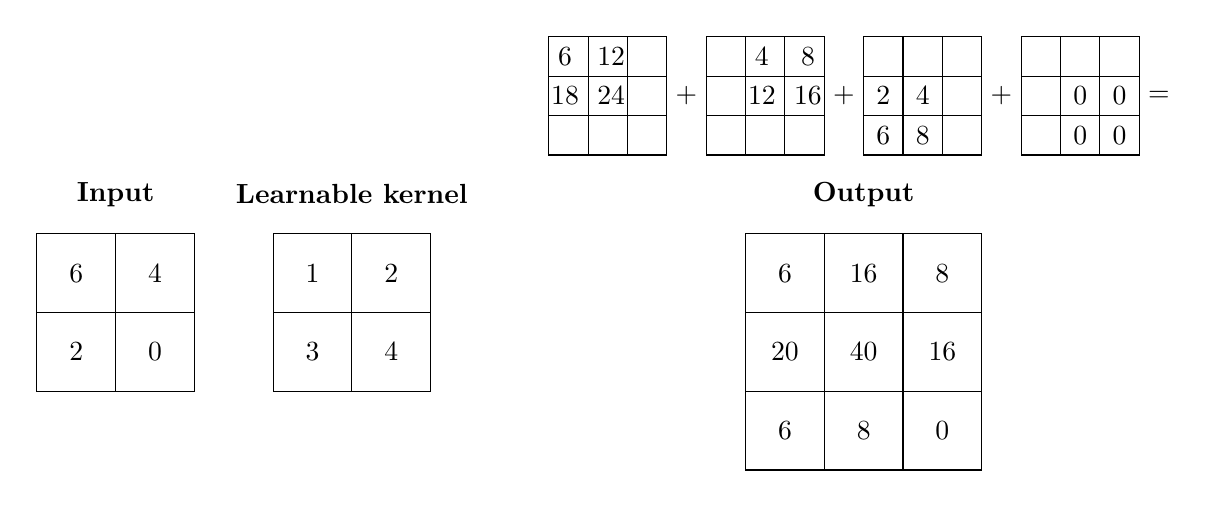
\begin{tikzpicture}
        % Input
        \node at (0, 0.5) {\textbf{Input}};

        \draw [fill=white] (-1,-2) rectangle ++(2,2) [step=1] grid ++(-2,-2);

        \matrix (m1) [matrix of nodes, ampersand replacement=\&, nodes={anchor=center, minimum size=1cm}] at (0, -1)
        {
            6 \& 4 \\
            2 \& 0 \\
        };

        % Kernel
        \node at (3, 0.5) {\textbf{Learnable kernel}};

        \draw [fill=white] (2,-2) rectangle ++(2,2) [step=1] grid ++(-2,-2);

        \matrix (m1) [matrix of nodes, ampersand replacement=\&, nodes={anchor=center, minimum size=1cm}] at (3, -1)
        {
            1 \& 2 \\
            3 \& 4 \\
        };

        % Small matrices
        \foreach \x in {5.5, 7.5, 9.5, 11.5}
            {
                \draw [fill=white] (\x,1) rectangle ++(1.5,1.5) [step=0.5] grid ++(-1.5,-1.5);
            }

        \node at (7.25, 1.75) {$+$};
        \node at (9.25, 1.75) {$+$};
        \node at (11.25, 1.75) {$+$};
        \node at (13.25, 1.75) {$=$};

        \matrix (m2) [matrix of nodes, ampersand replacement=\&, nodes={anchor=center, minimum size=0.5cm}] at (6.25, 1.75)
        {
            6 \& 12 \& ~  \\
            18 \& 24 \& ~ \\
            ~ \& ~ \& ~   \\
        };

        \matrix (m3) [matrix of nodes, ampersand replacement=\&, nodes={anchor=center, minimum size=0.5cm}] at (8.25, 1.75)
        {
            ~ \& 4 \& 8   \\
            ~ \& 12 \& 16 \\
            ~ \& ~ \& ~   \\
        };

        \matrix (m4) [matrix of nodes, ampersand replacement=\&, nodes={anchor=center, minimum size=0.5cm}] at (10.25, 1.75)
        {
            ~ \& ~ \& ~ \\
            2 \& 4 \& ~ \\
            6 \& 8 \& ~ \\
        };

        \matrix (m5) [matrix of nodes, ampersand replacement=\&, nodes={anchor=center, minimum size=0.5cm}] at (12.25, 1.75)
        {
            ~ \& ~ \& ~ \\
            ~ \& 0 \& 0 \\
            ~ \& 0 \& 0 \\
        };

        % Output
        \node at (9.5, 0.5) {\textbf{Output}};

        \draw [fill=white] (8, -3) rectangle ++(3,3) [step=1] grid ++(-3,-3);

        \matrix (m6) [matrix of nodes, ampersand replacement=\&, nodes={anchor=center, minimum size=1cm}] at (9.5, -1.5)
        {
            6 \& 16 \& 8   \\
            20 \& 40 \& 16 \\
            6 \& 8 \& 0    \\
        };

    \end{tikzpicture}

    Advantage: learnable approach\\
    Downside: can lead to "checkerboard artefacts" if the stride/size is not chosen correctly.
\end{frame}

\begin{frame}
    {Example - SegNet}
    \centering
    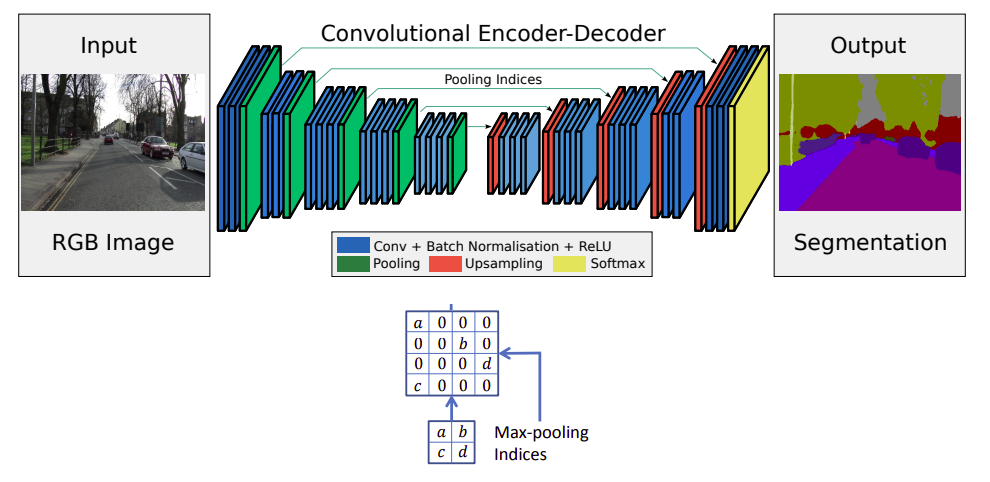
\includegraphics[width=\textwidth]{Badrinarayanan2016_segnet.png}

    \footnotesize
    Badrinarayanan, A., et al. \textbf{SegNet: A Deep Convolutional Encoder-Decoder Architecture for Image Segmentation}.
\end{frame}

\begin{frame}
    {U-Net - segmentation for biomedical images}
    \centering
    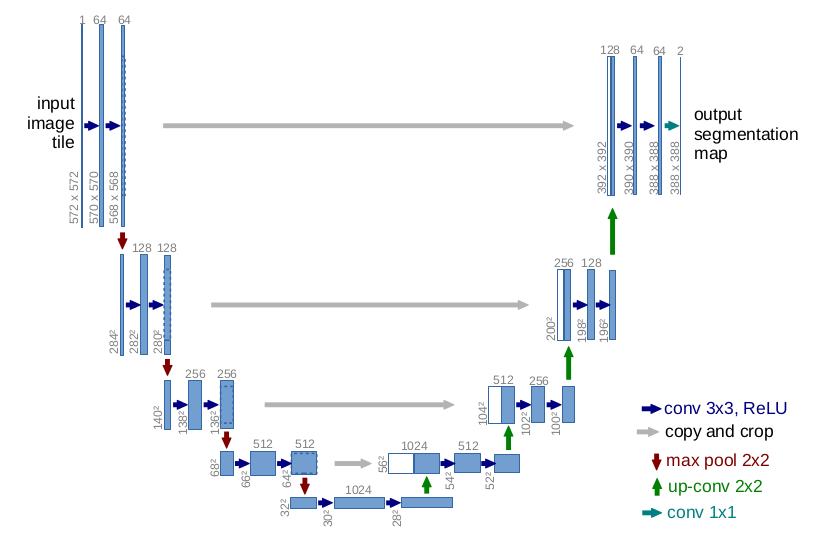
\includegraphics[width=.8\textwidth]{Ronneberger 2015 - UNet.png}

    \footnotesize
    Ronneberger et al., 2015 - U-Net: Convolutional Networks for Biomedical Image Segmentation
\end{frame}

\section {Localization and detection}

\begin{frame}
    {Localization}
    \textbf{Localization problem}: find the position of an object of interest in the image. We know that there is exactly one.

    For example, I want to find the position of a cell in an image, and define what type of cell that is.

    \vspace{3em}

    \centering
    \Large
    \textbf{How to do that?}
\end{frame}

\begin{frame}
    {CNN with multiple outputs}
    \begin{tikzpicture}
        \node[draw, inner sep=0pt] (image) at (0,0)
        {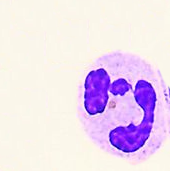
\includegraphics[height=2.5cm]{neutrophil.png}};

        % Conv layers
        \foreach \x [count=\N] in {2.5,3,...,5}
            {
                \node (layer\N) [draw, rectangle, fill=orange!50!yellow, minimum width=1, minimum height=3cm-0.4*\N cm] at (\x,0) {};
            }
        % FC layers
        \foreach \x [count=\N from 7] in {6,6.5}
            {
                \node (layer\N) [draw, rectangle, fill=blue!50!yellow, minimum width=1, minimum height=2.5cm-.1*\N cm] at (\x,0) {};
            }

        % Softmax
        \node (layer9) [draw, rectangle, fill=blue!50!yellow, minimum width=1, minimum height=1cm] at (8.5,2) {};
        \node (layer10) [draw, rectangle, fill=green!50!yellow, minimum width=1, minimum height=1cm] at (9,2) {};

        % Bbox
        \node (layer11) [draw, rectangle, fill=blue!50!yellow, minimum width=1, minimum height=1cm] at (8.5,-2) {};
        \node (layer12) [draw, rectangle, fill=green!50!yellow, minimum width=1, minimum height=1cm] at (9,-2) {};

        % Arrows
        \draw [->] (image) -- (layer1);
        \foreach \N [count=\Nn from 2] in {1,2,...,9}
            {
                \draw [->] (layer\N) -- (layer\Nn.west);
            }

        \draw [->] (layer8) -- (layer11) [->] -- (layer12);

        \node [text width=5em] at (10.5, 2) {\textbf{Softmax} \mbox{Neutrophil: 0.92} \mbox{Eosinophil: 0.05} \mbox{Lymphocyte: 0.01} \mbox{RBC: 0.00} \dots};

        \node [text width=5em] at (10.5, -2) {\textbf{Bounding box} \mbox{\{x, y, width, height\}}};
    \end{tikzpicture}

    This network will use two losses, one for the classification and one for the bounding box. We will have an hyperparameter to weight the two losses at training time.
\end{frame}

\begin{frame}
    {Which losses do we use for these problems?}
    \only<1>{
        \textbf{Classification}

        \begin{itemize}
            \item Most commonly function is the \textbf{cross-entropy} loss
            \item Often called \textbf{softmax loss}. This is actually a softmax activation followed by a cross-entropy loss!
            \item For binary problems a variant is the \textbf{binary cross-entropy}
        \end{itemize}

        Cross entropy is defined as

        \Large
        $$L(y, \hat{y}) = -\sum_i y_i\log(\hat{y}_i)$$

        \normalsize
        where $\hat{y}_i$ is the predicted probability of the $i$-th class and $y$ is the ground truth.
    }
    \only<2>{
        \textbf{Bounding box}
        We can treat this as a regression problem and use a \textbf{mean squared error loss} (also called \textbf{$\mathbf{L_2}$ loss}).

        \Large

        $$L(y, \hat{y}) = \frac{1}{2} \sum_i (y_i - \hat{y}_i)^2$$
    }
\end{frame}

\begin{frame}
    {The detection problem}
    \centering
    What if we have multiple objects?

    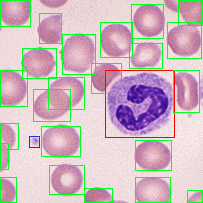
\includegraphics[width=.4\textwidth]{objectdetection.png}

    Problematic, as we don't know how many, if any, objects we are looking for!
\end{frame}

\begin{frame}
    {Cropping the image}
    A simple idea is to generate several crops of the image, and classify them separately.

    \centering
    \begin{tikzpicture}
        \node[draw, inner sep=0pt] (image) at (0,0)
        {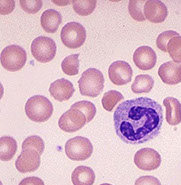
\includegraphics[height=2.5cm]{objectdetection_nobbox.png}};

        % Bounding boxes
        \node (crop1) [draw, rectangle, color=red, very thick, minimum height=0.6cm, minimum width=0.65cm] at (0.6,-0.4) {};

        \node (crop2) [draw, rectangle, color=blue, very thick, minimum size=0.3cm] at (-0.6,0.6) {};

        % CNN
        \node (CNN) [draw, fill=lightgray, minimum size=2cm] at (3, 0) {CNN};

        \draw [->, color=red] (crop1) -- (CNN);
        \draw [->, color=blue] (crop2) -- (CNN);

        \node [color=blue, text width=5em] at (5, 0) {\mbox{Neutrophil: 0.1} \mbox{Platelet: 0.05} \mbox{Lymphocyte: 0.01} \mbox{RBC: 0.84} \mbox{Background:0} + \mbox{\{0.2, 0.2, 0.1, 0.1\}}};
        \node [color=red, text width=5em] at (8, 0) {\mbox{Neutrophil: 0.96} \mbox{Platelet: 0.02} \mbox{Lymphocyte: 0.01} \mbox{RBC: 0.01} \mbox{Background:0} + \mbox{\{0.6, 0.6, 0.3, 0.25\}}};
    \end{tikzpicture}

    \vspace{2em}
    \textbf{Problem: how do I choose the crops?}
\end{frame}

\begin{frame}
    {R-CNN}
    \begin{itemize}
        \item R-CNN: region proposals + CNN
        \item Generates ~2000 regions
        \item The original paper uses the "selective search" algorithm, but R-CNN works with any other region searching algorithm
        \item Crops for the selected regions are passed through a CNN
    \end{itemize}
    \centering
    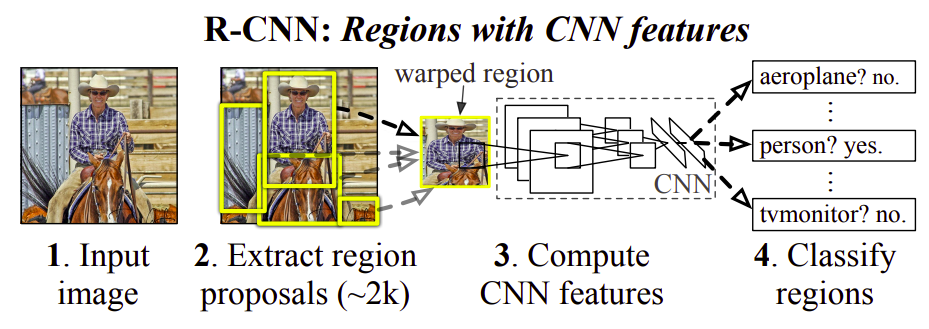
\includegraphics[width=.8\textwidth]{Girshick_2014_RCNN.png}

    \raggedright
    \footnotesize
    Girshick et al. 2014

    \normalsize
    Region proposal is fast (few seconds), but passing 2000 regions to a CNN is still time consuming.
\end{frame}

\begin{frame}
    {Fast R-CNN}
    \begin{itemize}
        \item We propose regions as in R-CNN
        \item We pass the whole image through a CNN only once
        \item We can then crop the feature map using the proposed regions saving a lot of computation!
        \item ~10x faster at training time, 150x faster at run time!
    \end{itemize}
    \centering
    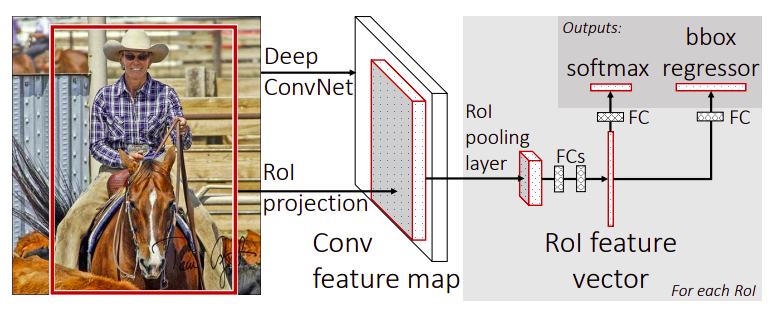
\includegraphics[width=\textwidth]{Girshick_2015_FastRCNN.png}

    \footnotesize
    Girshick, 2015
\end{frame}

\begin{frame}
    {Faster R-CNN}
    \begin{itemize}
        \item We pass the whole image through a CNN
        \item We learn regions from the feature map using a fully convolutional network
        \item We then crop the feature map as in Fast R-CNN
        \item 200+ times faster than R-CNN
    \end{itemize}
    \centering
    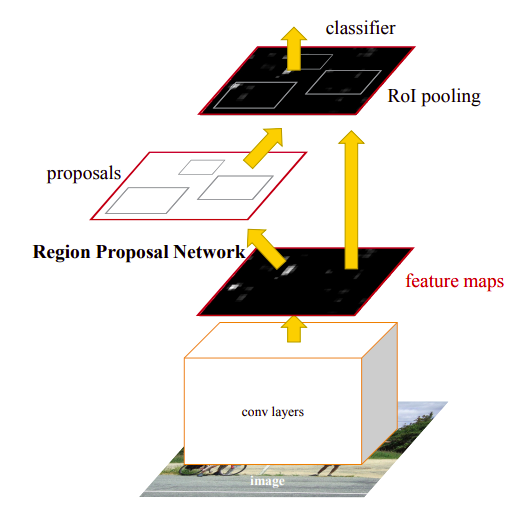
\includegraphics[width=.4\textwidth]{Ren_2016_faster_rcnn.png}

    \footnotesize
    Ren et al., 2016
\end{frame}

\begin{frame}
    {YOLO}
    \begin{itemize}
    \item YOLO splits the image into a grid of cells
    \item For each cell it generate a series of bounding boxes prediction and a class probability
    \item It's a one-shot method, so very fast!
    \item Strong spatial contstraints. Each cell can only predict a single object. 
    \end{itemize}
    \centering
    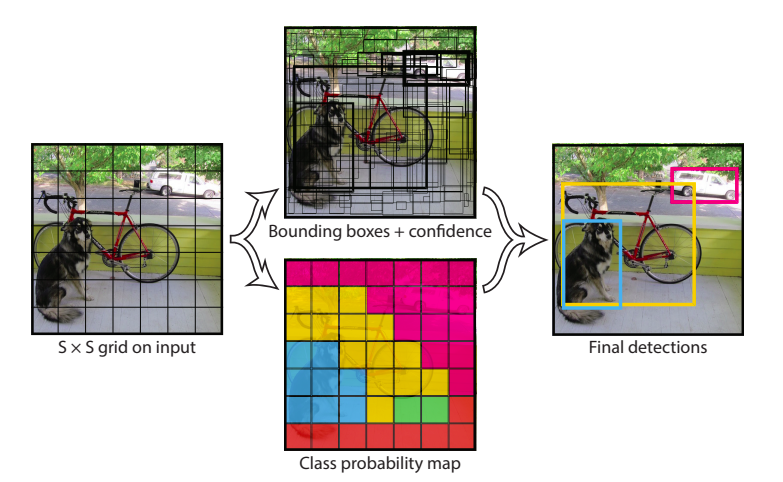
\includegraphics[width=.6\textwidth]{Redmon2016_YOLO.png}

    \footnotesize
    Redmon et al., 2016
\end{frame}

\begin{frame}
    {A final example: Stardist for cell segmentation}
    The UNet architecture has been heavily used and modified. For example, the Stardist network is a modification of the UNet architecture for 2D and 3D segmentation of cells.

    \centering
    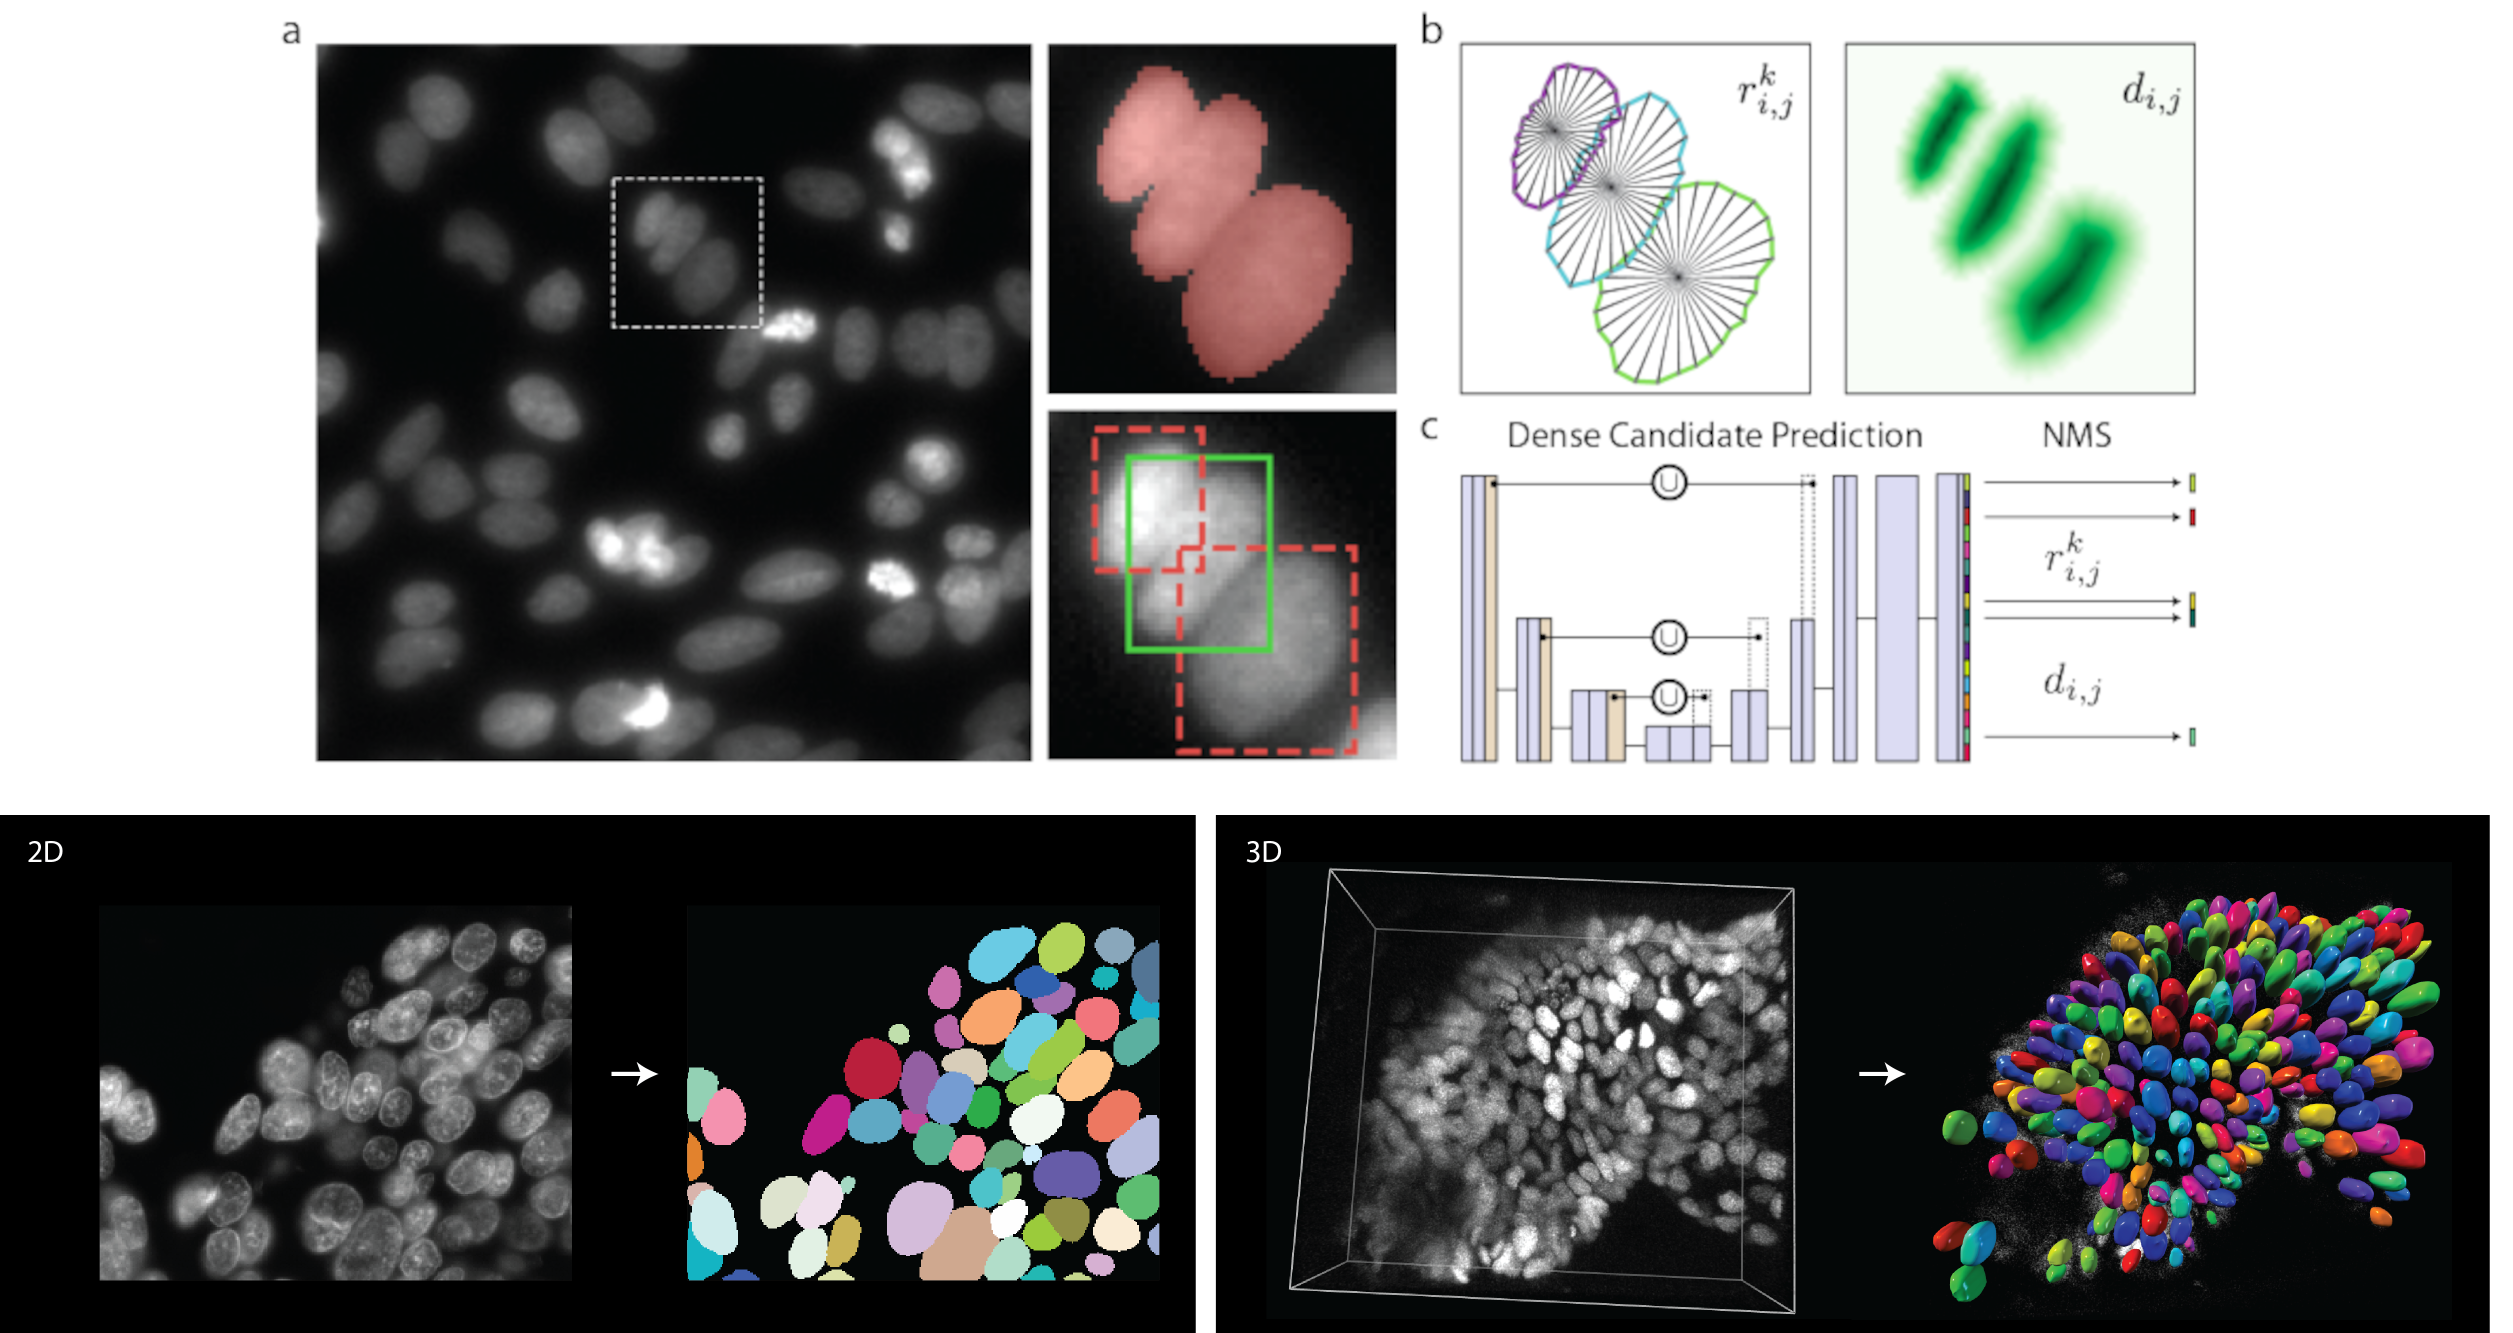
\includegraphics[width=.7\textwidth]{stardist.png}

    Schmidt et al. - Cell Detection with Star-convex Polygons.
    Weigert et al. - Star-convex Polyhedra for 3D Object Detection and Segmentation in Microscopy.
\end{frame}
\end{document}

